\documentclass[a4paper,12pt]{article}
\usepackage[top = 2.5cm, bottom = 2.5cm, left = 2.5cm, right = 2.5cm]{geometry}
\usepackage[T1]{fontenc}
\usepackage[utf8]{inputenc}
\usepackage{multirow} 
\usepackage{booktabs} 
\usepackage{graphicx}
\usepackage[spanish]{babel}
\usepackage{setspace}
\setlength{\parindent}{0in}
\usepackage{float}
\usepackage{fancyhdr}
\usepackage{amsmath}
\usepackage{amssymb}
\usepackage{amsthm}
\usepackage[numbers]{natbib}
\newcommand\Mycite[1]{%
	\citeauthor{#1}~[\citeyear{#1}]}
\usepackage{graphicx}
\usepackage{subcaption}
\usepackage{booktabs}
\usepackage{etoolbox}
\usepackage{minibox}
\usepackage{hyperref}
\usepackage{xcolor}
\usepackage{pdfpages}
\usepackage[skins]{tcolorbox}
%---------------------------

\newtcolorbox{cajita}[1][]{
	 #1
}

\newenvironment{sol}
{\renewcommand\qedsymbol{$\square$}\begin{proof}[\textbf{Solución.}]}
	{\end{proof}}

\newenvironment{dem}
{\renewcommand\qedsymbol{$\blacksquare$}\begin{proof}[\textbf{Demostración.}]}
	{\end{proof}}

\newtheorem{problema}{Problema}
\newtheorem{definicion}{Definición}
\newtheorem{ejemplo}{Ejemplo}
\newtheorem{teorema}{Teorema}
\newtheorem{corolario}{Corolario}[teorema]
\newtheorem{lema}[teorema]{Lema}
\newtheorem{prop}{Proposición}
\newtheorem*{nota}{\textbf{NOTA}}
\renewcommand\qedsymbol{$\blacksquare$}
\usepackage{svg}
\usepackage{tikz}
\usepackage[framemethod=default]{mdframed}
\global\mdfdefinestyle{exampledefault}{%
linecolor=lightgray,linewidth=1pt,%
leftmargin=1cm,rightmargin=1cm,
}




\newenvironment{noter}[1]{%
\mdfsetup{%
frametitle={\tikz\node[fill=white,rectangle,inner sep=0pt,outer sep=0pt]{#1};},
frametitleaboveskip=-0.5\ht\strutbox,
frametitlealignment=\raggedright
}%
\begin{mdframed}[style=exampledefault]
}{\end{mdframed}}
\newcommand{\linea}{\noindent\rule{\textwidth}{3pt}}
\newcommand{\linita}{\noindent\rule{\textwidth}{1pt}}

\AtBeginEnvironment{align}{\setcounter{equation}{0}}
\pagestyle{fancy}

\fancyhf{}









%----------------------------------------------------------
\lhead{\footnotesize Data Science I}
\rhead{\footnotesize  Rudik Roberto Rompich}
\cfoot{\footnotesize \thepage}


%--------------------------

\begin{document}
 \thispagestyle{empty} 
    \begin{tabular}{p{15.5cm}}
    \begin{tabbing}
    \textbf{Universidad del Valle de Guatemala} \\
    Departamento de Ciencias de la Computación\\\\
   \textbf{Estudiantes:} Augusto Alonso, Angel Cuellar, Rudik Roberto Rompich\\
    \end{tabbing}
    \begin{center}
        CC3066 - Data Science I - Catedrático: Luis Furlan\\
        \today
    \end{center}\\
    \hline
    \\
    \end{tabular} 
    \vspace*{0.3cm} 
    \begin{center} 
    {\Large \bf  Proyecto 2 - Análisis Exploratorio 
} 
        \vspace{2mm}
    \end{center}
    \vspace{0.4cm}
%--------------------------

\textbf{Instrucciones:} 

Para este ejercicio, trabajarán con 4 conjuntos de datos:
\begin{enumerate}
	\item daily-total-female-births.csv
	\item shampoo.csv
	\item monthly-car-sales.csv
	\item monthly-mean-temp.csv
\end{enumerate}
Cada uno de estos conjuntos representan series de tiempo, pero muestran diferentes características relacionadas con la tendencias, estacionalidad, período, etc. (ver presentación de clase)

Hemos visto 5 métodos diferentes para predecir con series de tiempo, a decir:  
\begin{enumerate}
	\item Promedio (para usar como base de referencia)
	\item SARIMAX
	\item Alisamiento exponencial (Winter-Holt)
	\item Red Neuronal
	\item FB Prophet
\end{enumerate}

En este laboratorio, deben ejecutar los 5 métodos para cada uno de los conjuntos de datos arriba indicados.

%---------------------
\begin{problema}
	Utilizando la prueba del RMSE (raíz cuadrada de la media de los errores alcuadrado).  Generen gráficas para el caso que dió el mejor resultado de cada método en cada conjunto de datos.
\end{problema}

%----------------------
\begin{problema}
	¿Qué métodos logran captar mejor las tendencias y las variaciones estacionales?
\end{problema}

%----------------------
\begin{problema}
	Generen una tabla comparativa que muestre los RMSE más bajos para cada método con cada conjunto de datos. En la tabla indiquen qué método fue mejor para cada caso de datos.  Por ejemplo:
	\begin{figure}
		\centering
		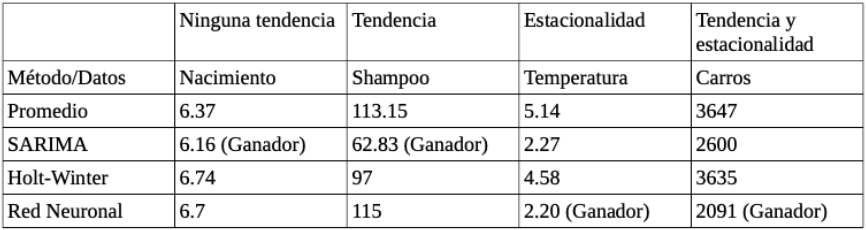
\includegraphics[scale=0.5]{Images/1}
	\end{figure}
\end{problema}

%----------------------
\begin{problema}
	Ahora apliquen el FB Prophet con cada uno de los conjuntos de datos. Compare los resultados con los de los métodos anteriores.  ¿Hay algún ganador claro, entre todos los métodos?
\end{problema}


%----------------------
\begin{problema}
	 Escriban sus conclusiones sobre lo aprendido en este módulo sobre seriesde tiempo.  ¿Cuál es el mejor procedimiento para resolver un problema de predicción de series de tiempo?  
\end{problema}



%---------------------------
\bibliographystyle{apa}
\bibliography{referencias.bib}

\end{document}